\tikzset{every picture/.style={line width=0.75pt}} %set default line width to 0.75pt        

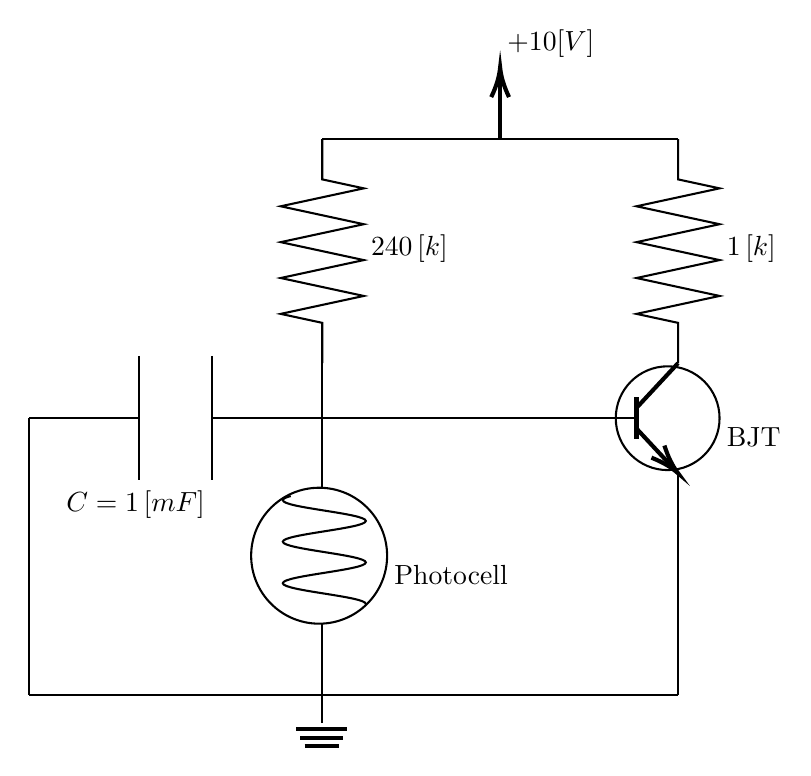
\begin{tikzpicture}[x=0.75pt,y=0.75pt,yscale=-1,xscale=1]
%uncomment if require: \path (0,497); %set diagram left start at 0, and has height of 497

%Shape: Resistor [id:dp08557489822351128] 
\draw   (214,71) -- (214,90.44) -- (234,94.76) -- (194,103.4) -- (234,112.04) -- (194,120.68) -- (234,129.32) -- (194,137.96) -- (234,146.6) -- (194,155.24) -- (214,159.56) -- (214,179) ;
%Straight Lines [id:da10613850567534644] 
\draw    (355.42,205.5) -- (214,205.5) ;
%Shape: Resistor [id:dp42863709400980965] 
\draw   (385.42,71) -- (385.42,90.44) -- (405.42,94.76) -- (365.42,103.4) -- (405.42,112.04) -- (365.42,120.68) -- (405.42,129.32) -- (365.42,137.96) -- (405.42,146.6) -- (365.42,155.24) -- (385.42,159.56) -- (385.42,179) ;
%Shape: Circle [id:dp6263492261348075] 
\draw   (355.42,205.5) .. controls (355.42,191.69) and (366.61,180.5) .. (380.42,180.5) .. controls (394.23,180.5) and (405.42,191.69) .. (405.42,205.5) .. controls (405.42,219.31) and (394.23,230.5) .. (380.42,230.5) .. controls (366.61,230.5) and (355.42,219.31) .. (355.42,205.5) -- cycle ;
%Straight Lines [id:da5434466420085665] 
\draw    (365.42,205.5) -- (355.42,205.5) ;
%Straight Lines [id:da8222789328378522] 
\draw [line width=1.5]    (365.42,215.5) -- (365.42,195.5) ;
%Straight Lines [id:da6868248647799469] 
\draw [line width=1.5]    (365.42,210.5) -- (383.38,229.8) ;
\draw [shift={(385.42,232)}, rotate = 227.07] [color={rgb, 255:red, 0; green, 0; blue, 0 }  ][line width=1.5]    (14.21,-4.28) .. controls (9.04,-1.82) and (4.3,-0.39) .. (0,0) .. controls (4.3,0.39) and (9.04,1.82) .. (14.21,4.28)   ;
%Straight Lines [id:da7170401481045089] 
\draw [line width=1.5]    (385.42,179) -- (365.42,200.5) ;
%Straight Lines [id:da09379764529365986] 
\draw    (385.42,339) -- (214,339) ;
%Straight Lines [id:da37329225941611255] 
\draw    (385.42,71) -- (214,71) ;
%Straight Lines [id:da20374241030260287] 
\draw [line width=1.5]    (299.71,71) -- (299.71,39.58) ;
\draw [shift={(299.71,36.58)}, rotate = 90] [color={rgb, 255:red, 0; green, 0; blue, 0 }  ][line width=1.5]    (14.21,-4.28) .. controls (9.04,-1.82) and (4.3,-0.39) .. (0,0) .. controls (4.3,0.39) and (9.04,1.82) .. (14.21,4.28)   ;
%Straight Lines [id:da09982064594930351] 
\draw [line width=0.75]    (213.71,352.42) -- (213.71,339) ;
%Straight Lines [id:da7825511264162391] 
\draw [line width=1.5]    (201.5,355.42) -- (225.92,355.42) ;
%Straight Lines [id:da8263231613187413] 
\draw [line width=1.5]    (203.5,359.42) -- (223.92,359.42) ;
%Straight Lines [id:da4438946372208784] 
\draw [line width=1.5]    (205.5,363.42) -- (221.92,363.42) ;
%Straight Lines [id:da9620365649992906] 
\draw    (214,339) -- (72.58,339) ;
%Straight Lines [id:da22791584371112872] 
\draw    (72.58,205.5) -- (72.58,339) ;
%Straight Lines [id:da8821366946228647] 
\draw    (214,179) -- (214,205.5) ;
%Shape: Contact [id:dp522587048630987] 
\draw   (99.08,205.5) -- (125.61,205.5) (187.5,205.5) -- (160.97,205.5) (125.61,175.5) -- (125.61,235.5) (160.97,175.5) -- (160.97,235.5) ;
%Straight Lines [id:da5619511756017568] 
\draw    (214,205.5) -- (187.5,205.5) ;
%Straight Lines [id:da6523589746503576] 
\draw    (99.08,205.5) -- (72.58,205.5) ;
%Straight Lines [id:da7347230772485945] 
\draw    (214,204.5) -- (214,239) ;
%Straight Lines [id:da6427167659637599] 
\draw    (385.42,232) -- (385.42,339) ;
%Straight Lines [id:da8613521999063483] 
\draw    (214,304.5) -- (214,339) ;
%Shape: Circle [id:dp050443532359439325] 
\draw   (179.75,271.75) .. controls (179.75,253.66) and (194.41,239) .. (212.5,239) .. controls (230.59,239) and (245.25,253.66) .. (245.25,271.75) .. controls (245.25,289.84) and (230.59,304.5) .. (212.5,304.5) .. controls (194.41,304.5) and (179.75,289.84) .. (179.75,271.75) -- cycle ;
%Shape: Wave [id:dp9314080913049783] 
\draw   (198.82,243) .. controls (196.45,243.64) and (195,244.3) .. (195,245) .. controls (195,246.81) and (204.75,248.37) .. (215,250) .. controls (225.25,251.63) and (235,253.19) .. (235,255) .. controls (235,256.81) and (225.25,258.37) .. (215,260) .. controls (204.75,261.63) and (195,263.19) .. (195,265) .. controls (195,266.81) and (204.75,268.37) .. (215,270) .. controls (225.25,271.63) and (235,273.19) .. (235,275) .. controls (235,276.81) and (225.25,278.37) .. (215,280) .. controls (204.75,281.63) and (195,283.19) .. (195,285) .. controls (195,286.81) and (204.75,288.37) .. (215,290) .. controls (225.25,291.63) and (235,293.19) .. (235,295) ;

% Text Node
\draw (301.71,33.18) node [anchor=south west] [inner sep=0.75pt]    {$+10[ V]$};
% Text Node
\draw (407.42,208.5) node [anchor=north west][inner sep=0.75pt]   [align=left] {BJT};
% Text Node
\draw (407.42,115.44) node [anchor=north west][inner sep=0.75pt]    {$1\left[\text{k} \si{\ohm}\right]$};
% Text Node
\draw (236,115.44) node [anchor=north west][inner sep=0.75pt]    {$240\left[\text{k} \si{\ohm}\right]$};
% Text Node
\draw (158.97,238.9) node [anchor=north east] [inner sep=0.75pt]    {$C=1\left[\text{mF}\right]$};
% Text Node
\draw (247.25,274.75) node [anchor=north west][inner sep=0.75pt]   [align=left] {Photocell};


\end{tikzpicture}
